
\chapter{Methods}
This project aims to enhance AstaZero's documentation of Euro NCAP tests conducted at their test facility, specifically tests that require aerial documentation by use of drones.

\section{Project setup and structure}
The team was comprised of students from both Chalmers University of Technology
and Penn State University. There were six students from Chalmers University with
majors in Mechanical Engineering and Automation and Mechatronics, with three
students in each major. Furthermore, there were six students from Penn State University with diverse majors, Mechanical Engineering (3), Computer Science (1), and Computer Engineering (2). This diversification in educational foundation provided complementing strengths that were applied during the project.

The primary objective of the project was to develop an android application. Said app would facilitate communication between the drones and the control system (ATOS), both supplied by AstaZero. However, there were some things in the ATOS softwarethat  needed to be modified and added in order for it to work. AstaZero had already developed an Android application with limited functionality that had basic features that allowed communication with the drone. The objective was to keep developing this app to give it more features and automate it. The main objective of the project was software development and did not involve any physical construction. However, as outlined in chapter \ref{chap:demarcation}, there were plans to incorporate hardware development if adequate time was available.

The team documented and wrote the report during all phases of the project. To keep track of all the different tasks and what tasks were assigned to whom, the application Trello was used as a project management board. Within the project, different persons had different roles. Some were project managers responsible for the reports, administration, Trello board and deadlines, and some focused more on developing the application. Figure \ref{fig:workflow} showed how the work had been divided into different phases of the project.



\begin{figure}[H]
  \centering
  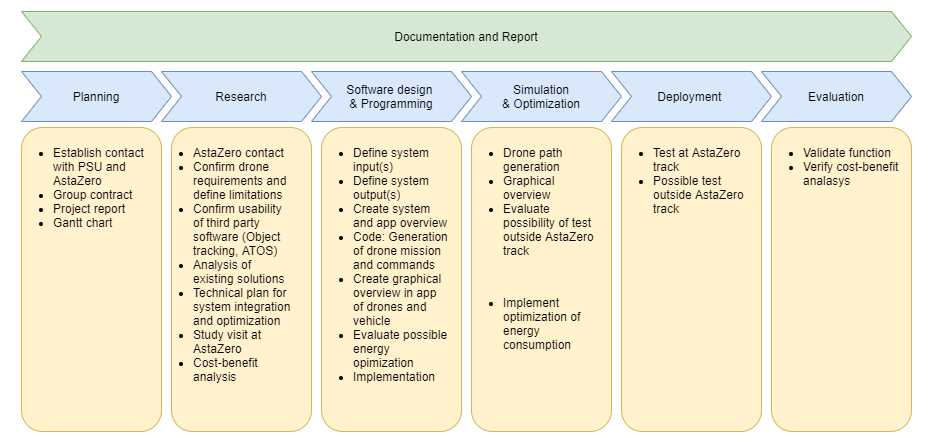
\includegraphics[width=\columnwidth]{figure/work_flow.png}
  \caption{Work flow of the project}
  \label{fig:workflow}
\end{figure}

\subsection{Work distribution between the two universities}
As previously stated, the Bachelor's Thesis was conducted as a joint venture between Chalmers University of Technology and Pennsylvania State University. Due to the time difference between the two universities, it was crucial to clearly define the division of labor. This facilitated consistent and independent work from each group, eliminating the need for constant communication.
\\

For the configuration to function properly, two pieces of software needed to be developed and integrated: ATOS and the drone app. This setup allowed for a natural division of labor between the universities, as both the app and ATOS, which had already been developed by AstaZero, could be worked on independently.
\\

Accordingly, the Chalmers team was solely responsible for developing the drone app, while the PSU team handled the orchestration of the test objects (ATOS) and path calculations. However, since both ATOS and the app were equally crucial for the success of the project, and equally essential for the configuration to even operate, both groups had to be held accountable for upholding their part of the project.

\section{Analysis}
\todo{Är detta överflödigt?}
In order to compile a complete understanding of the project parameters and objectives, an analysis of the critical parts needed to be conducted beforehand. The critical parts were defined as parts that had the possibility to significantly alter the outcome of the project. The drone capabilities and limitations were assessed in relation to the Euro NCAP test. A clear and extensive comprehension of the ATOS software and communication protocols was obtained, as well as the requirements for the android app. The level of robustness of the drone software was determined, in other words, what magnitude of interference the software was capable of regulating without losing its functionality.

\section{Scoping and information gathering}
Research and information gathering were conducted continuously throughout the project and encompassed the majority of the project's initial workload. The research commenced with the introduction given by Victor Jarlow, the point of contact at AstaZero. This presentation gave crucial information on how a Euro NCAP trial was performed at the test site, the AV test control system used, as well as the project parameters and goals.

%\subsection{Euro NCAP tests}
%As per the problem statement stated in \ref{chap:problem statement}, the software is supposed to be used to film various tests conducted under the Euro NCAP specifications. The team both at PSU and Chalmers quickly decided to only focus at one test at first and expand to all tests afterwards if time allowed it. The test selected was the Autonomous emergency breaking tests - VRU outlined in section 10 of the Euro NCAP Film and Photo Protocol \cite{EuroNCAP2021EUROPEANPROTOCOL}. This test requires the use of a drone and the protocol clearly states where the drone is supposed to be at all times, making it a good test to begin with.



%\subsection{AV testing operating system (ATOS)}
%The core of each test is ATOS, short for Autonomous Vehicle Testing Operating
%System, which follows different standards developed by AstaZero and creates paths
%for each object that is part of the test. An extensive comprehension of the ATOS
%software needs to be obtained, this includes the functional requirements, software
%specifications and the communication protocol. The information can be obtained in
%one of the documents provided by AstaZero (ISO DTS 22133). The integration of
%ATOS is illustrated in Figure~\ref{fig:ATOS}


%\subsection{AstaZero facility}
%In the early stages of the project, a study visit at the AstaZero test track was conducted. This study visit allowed the project group to obtain detailed specifications about the test facility, as well as possible consultation about the project with facility employees. Questions were prepared in advance for optimal information gathering.

%\section{Client requirements}
%The client’s requirements and wishes were stated in chapter \ref{chap:problem statement}. The course of action was to ensure the completion of the project’s main objectives. However, fulfillment of AstaZero’s wishes was taken into consideration during every stage of the project in order to achieve the best possible result. Furthermore, there were a few more aspects to keep in mind, more specifically regarding the safety. For instance, if there were some tests that required documentation during high speed, the drones may have needed to go into sports-mode which disabled some of the drones' built-in safety features, such as automatic object detection. This increased the risk of failure, and therefore, the project had to be executed with caution and precision to ensure that the objectives, wishes and safety requirements were met to the maximum extent.

%In addition to the requirements stated earlier, the client expressed a wish for the report to incorporate a cost-benefit analysis pertaining to the adoption of the drone and app configuration. This analysis comprised both reasoning and quantification of the net present value to appraise the investment. The options were weighed out and evaluated in both monetary as well as non-monetary regards. 



\section{Test driven development}
Throughout the duration of the project, the software development methodology known as Test-Driven Development (TDD) has been a source of inspiration for this project. TDD is a process that follows an iterative development cycle and involves the creation of tests before writing the code itself. As a component of the agile software development approach, TDD emphasizes continuous integration, testing, and deployment ~\cite{WhatTestDriven.io}.

In order to ensure the robustness of each subsystem of the drone application, it was crucial to continuously test them. This approach helped to facilitate a smoother integration process, while also providing ease in identifying any subsystem failures.

TDD is based on three fundamental principles: red, green, refactor. The chart detailing this process is provided in figure \ref{fig:TDD}. 
\\

\begin{figure}[H]
  \centering
  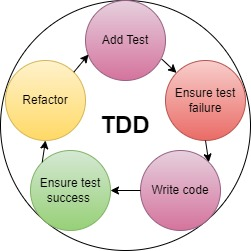
\includegraphics[width=0.5\textwidth]{figure/TDD.jpg}
  \caption{Test driven development}
  \label{fig:TDD}
\end{figure}

Throughout the project, the application of TDD has proved to be highly advantageous in the development of the app, with the team setting a predefined goal for each function. The difference between this development process and TDD is that the tests consisted of actual flight and gimbal movements instead of software tests. Its modular approach to code development and ease for step-by-step improvement have made the code easier to maintain. 

\section{Code development
\todo{Borde handla om ett övergripande tillvägagångsätt för mjukvarutvecklingen}
The app should allow the drone to receive predetermined flight paths, trajectories, from ATOS and to fly along these trajectories on command. During a real test carried out by AstaZero, these trajectories will closely resemble the tested vehicles trajectories to allow the drone to film the vehicle up close. To ensure desired video quality, the drone should consistently check and adjust the angle of its camera to keep the tested vehicle in the middle of the frame. We assigned the first task of processing and flying along trajectories to one part of our group and the other task of image recognition and adjustment of the drone’s camera angle to another part of the group. The two different projects should later on be merged to provide the full functionality of the app.
\subsection{Image recognition}
Image recognition and camera positioning:
Different solutions to the task of image recognition were proposed earlier in our work, but we  learned from the sponsor that the DJI SDK comes with some functions to track an object, meaning recognising an object and adjusting the gimbal (the robotic arm controlling the camera angle) to keep said object in focus. These functions turned out to be rather sophisticated and efficient meaning our concerns of the drone not having enough computing power to quickly adapt to changes in the vehicle’s and drone’s positions ceased. This is the guide that was used https://developer.dji.com/mobile-sdk/documentation/android-tutorials/P4MissionsDemo.html . \todo{Såhär kan vi inte skriva, vi får referera istället //MS} The code from this guide was combined with a folder supplied by AstaZero which contained an early app that could communicate with the drone. After a couple of tweaks most of the desired functionality worked, the drone recognised objects and stayed in place while adjusting its rotation to keep the chosen recognised object in the center of the video feed. The goal was for the drone to adjust the gimbal, not the drone’s rotation to keep the object in its camera’s center, but code to adjust the gimbal from the other app was believed to be able to solve this issue.